\section{Adatbázisok}
\paragraph{}
Adatbázisnak nevezzük azokat a nagy mennyiségű adatokat amelyek közös jellemzőkkel és struktúrákkal rendelkeznek. Az adatbázisokon belül több fajta műveletet tudunk elvégezni: karbantartás, tárolás, lekérdezés, szerkesztés, módosítás és nem utolsó sorban az adatok törlése is egy lehetőség. Ezen funkciókat egy adatbázis kezelő rendszer segítségével tudjuk elvégezni.\cite{dbms} Azonban különbséget kell tennünk az SQL (Structured Query Language) és a NoSQL(Not only Structured Query Language) között.
\subsection{SQL(Structured Query Language)}
\paragraph{}
Az elmúlt harminc évben a relációs adatbázis volt az alapértelmezett strukturált adatlekérdezési nyelv. Világunk fejlődése miatt egyre több és nagyobb információ adatok robbantak ki így az SQL alapú adatlekérdezés elveszítette hatékonyságát ezzel maga elé állítva azt a kihívást, hogy a nagyobb adatbázisok kezelése jóval megnehezedett. Ebből kifolyólag lehet arra következtetni hogy az SQL alapú szerverek hajlamosak nagy mennyiségű memóriát foglalni, biztonsági kockázatokat és teljesítményproblémákat elkövetni.\cite{venkatraman2016sql} 
	
\subsection{NoSQL(Not only Structured Query Language)}
\paragraph{}
A NoSQL adatbázisokat azért alkották meg, hogy az SQL adatbázisok által felfedezett hibákat orvosolják. Ezek az adatbázisok sokkal rugalmasabbak lettek, fő céljuk az adatok könnyű tárolása és visszakeresése függetlenül a szerkezetektől és tartalomtól. Automatikusan kezelik az adatkezelést, hibajavítást amelyek költségmegtakarítás szempontjából is fontosak.\cite{venkatraman2016sql} 
	
\subsection{SQL vs NoSQL}
\paragraph{}
A relációs adatbázisok az egyszerűség miatt leggyakoribb adatbázistípusok. Az adatok több táblára vannak bontva amelyekhez egyszerűen hozzá lehet férni. Az olyan műveletek, mint összeadás, létrehozás, visszakeresés, törlés stb. nagyon egyszerűen elvégezhetőek az SQL által megadott szintaxisok betartásával. Ilyen típusú adatbázis kezelő rendszerek a következőek: Oracle, SQL Server, MySQL, PostgreSQL stb. A folyamatos adatmennyiség miatt a relációs adatbázisok hátrányba kerültek a nem relációs adatbázisokkal szemben. A nem relációs adatbázisok sokkal gyorsabban és hatékonyabban tudják elvégezni feladataikat mint a relációsak. Nem relációs adatbázis típusú rendszerek a következőek lehetnek: Firebase, MongoDB, GraphQL stb.\cite{gupta2017nosql} A tanulmányok sokat segítenek abban, hogy egy adott projektben relációs vagy nem relációs adatbázist használjunk. Ha sok adatunk van és törekedünk a hatékonyságra akkor érdemesebb a nem relációs adatbázisokat használni. 
\paragraph{}
Több tanulmány is szól az adatbázisok teljesítményéről. A következőkben bemutatnék egyet. Ebben a tanulmányban három tesztet végeztek el. A kísérletben szerepelnek a következő adatbázis kezelő rendszerek: Cassandra, HBase, Memcached, MongoDb, OrientDB, Redis és a Voldemort.\cite{martins2019study} Az első tesztben 6.000.000 rekord állt az adatbázis kezelők rendelkezésére. A munkaterhelés fele olvasást és fele frissítést tartalmazott. Az eredmény a \ref{fig:performance_a} ábrán látható.
	
\begin{figure}
	\centering
	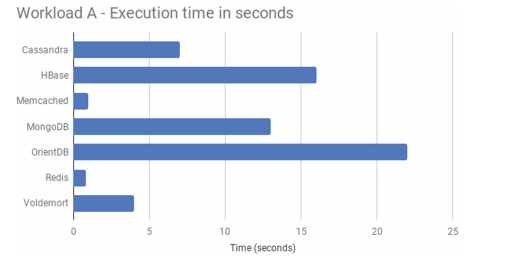
\includegraphics[scale=0.6]{figures/images/performance_a.png}
	\caption{Az adatbázis teljesítmény kísérlet első eredménye \cite{martins2019study}}
	\label{fig:performance_a}
\end{figure}

A második teszt szintén 6.000.000 rekordot tartalmazott. A munkaterhelés 5.000 véletlenszerű olvasás volt. Az eredmények \ref{fig:performance_b} ábrán láthatóak.
	
	\begin{figure}
		\centering
		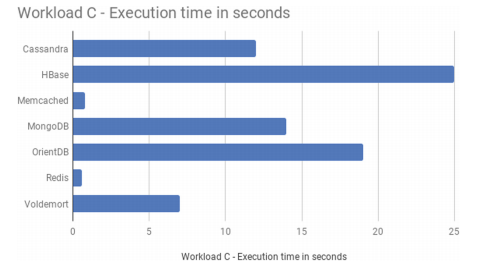
\includegraphics[scale=0.6]{figures/images/performance_b.png}
		\caption{Az adatbázis teljesítmény kísérlet második eredménye \cite{martins2019study}}
		\label{fig:performance_b}
	\end{figure}
	
A harmadik teszt szintén 6.000.000 rekordot tartalmazott. A munkaterhelés 5.000 véletlenszerű frissítés volt. Az eredmények \ref{fig:performance_c} ábrán láthatóak.
	
	\begin{figure}
		\centering
		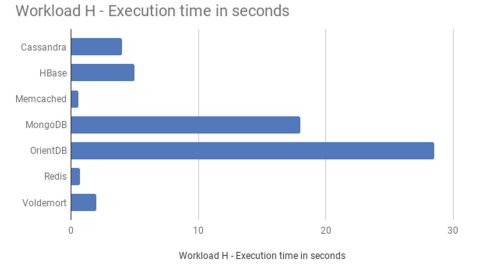
\includegraphics[scale=0.6]{figures/images/performance_c.png}
		\caption{Az adatbázis teljesítmény kísérlet harmadik eredménye \cite{martins2019study}}
		\label{fig:performance_c}
	\end{figure}